\documentclass[a4]{beamer}
\usepackage{amssymb}
\usepackage{graphicx}
\usepackage{subfigure}
\usepackage{newlfont}
\usepackage{amsmath,amsthm,amsfonts}
%\usepackage{beamerthemesplit}
\usepackage{pgf,pgfarrows,pgfnodes,pgfautomata,pgfheaps,pgfshade}
\usepackage{mathptmx}  % Font Family
\usepackage{helvet}   % Font Family
\usepackage{color}

\mode<presentation> {
 \usetheme{Default} % was Frankfurt
 \useinnertheme{rounded}
 \useoutertheme{infolines}
 \usefonttheme{serif}
 %\usecolortheme{wolverine}
% \usecolortheme{rose}
\usefonttheme{structurebold}
}

\setbeamercovered{dynamic}

\title[MathsCast]{Statistics for Computing \\ {\normalsize MA4413 Lecture 2A}}
\author[Kevin O'Brien]{Kevin O'Brien \\ {\scriptsize Kevin.obrien@ul.ie}}
\date{Autumn Semester 2012}
\institute[Maths \& Stats]{Dept. of Mathematics \& Statistics, \\ University \textit{of} Limerick}

\renewcommand{\arraystretch}{1.5}

\begin{document}

\begin{frame}
\titlepage
\end{frame}


%--------------------------------------------------------%
\frame{
\frametitle{Today's Class}
\begin{itemize}
\item Sampling without replacement.
\item Factorials
\item Permutations
\item Combinations
%\item Relative Frequency and Frequency tables
%\item Histograms
\item Sample mean
\item Median
\item Measures of dispersion
%\item Expected Values
\end{itemize}

}



\frame{
\frametitle{Sampling without replacement}
\begin{itemize}
\item Sampling is said to be ``without replacement" when a unit is selected at random from the population and it is not returned to the main lot. \item The first unit is selected out of a population of size $N$ and the second unit is selected out of the remaining population of  $N-1$ units and so on.
    \item For example, if you draw one card out of a deck of 52, there are only 51 cards left to draw from if you are selecting a second card.
\end{itemize}
}

\frame{
\frametitle{Sampling without replacement}
A lot of 100 semiconductor chips contains 20 that are defective.
Two chips are selected at random, without replacement from the lot.
\begin{itemize}
\item What is the probability that the first one is defective? \\(Answer : 20/100 , i.e 0.20)
\item What is the probability that the second one is defective given that the first one was defective? \\(Answer: 19/99)
\item What is the probability that the second one is defective given that the first one was not defective? \\(Answer: 20/99)
\end{itemize}
}

\frame{
\frametitle{Sampling With Replacement }

Sampling is called ``with replacement" when a unit selected at random from the population is returned to the population and then a second element is selected at random. Whenever a unit is selected, the population contains all the same units.
\begin{itemize}
\item What is the probability of guessing a PIN number for an ATM card at the first attempt.

\item Importantly a digit can be used twice, or more, in PIN codes.

\item For example $1337$ is a valid pin number, where $3$ appears twice.

\item
We have a one-in-ten chance of picking the first digit correctly, a one-in-ten chance of the guessing the second, and so on.

\item All of these events are independent, so the probability of guess the correct PIN is $0.1 \times 0.1 \times 0.1 \times 0.1 = 0.0001$
\end{itemize}
}
%--------------------------------------------------------%
\section{ Combinations and Permutations }

%--------------------------------------------------------%
\frame{
\frametitle{Factorials Numbers}

A factorial is a positive whole number, based on a number $n$ , and which is written as $``n!"$. The factorial $n!$ is defined as follows:

\[n!  =n \times (n-1) \times (n-2) \times \ldots \times 2 \times 1 \]

Remark $n!  =n \times (n-1)!$\\ \bigskip

\textbf{ Example: }

\begin{itemize}
\item $3!  = 3 \times 2  \times 1 = 6 $

\item $4!  = 4 \times 3! = 4 \times 3 \times 2 \times 1 = 24$
\end{itemize}
Remark $0! = 1$ not $0$.


}

%--------------------------------------------------------%
\frame{
\frametitle{Permutations and Combinations}


Often we are concerned with computing the number of ways of selecting and arranging groups of items. \begin{itemize} \item  A \textbf{\emph{combination}} describes the selection of items from a larger group of items.  \item A \textbf{\emph{permutation}} is a combination that is arranged in a particular way.
\end{itemize}

\bigskip
\begin{itemize}
\item Suppose we have items A,B,C and D to choose two items from.
\item AB is one possible selection, BD is another. AB and BD are both combinations.
\item More importantly, AB is one combination, for which there are two distinct permutations: AB and BA.
\end{itemize}
}

%--------------------------------------------------------%
\frame{
\frametitle{Combinations}

\textbf{Combinations: }
The number of ways of selecting $k$ objects from $n$ unique objects is:

\[ ^n C_k = {n!  \over k! \times (n-k)!} \]

In some texts, the notation for finding the number of possible combination is written

\[ ^n C_k =  {n \choose k} \]

}

%--------------------------------------------------------%
\frame{
\frametitle{Example of Combinations}
How many ways are there of selecting two items from possible 5?

\[ ^5 C_2   \left( \mbox{ also }  {5 \choose 2}  \right) =  {5!  \over 2! \times 3!} =  {5 \times 4 \times 3!  \over 2 \times 1 \times 3!} = 10  \]

\bigskip
Discuss how combinations can be used to compute the number of rugby matches for each group in the Rugby World Cup.

}
%--------------------------------------------------------%
\frame{
\frametitle{The Permutation Formula}
The number of different permutations of r items from n unique items is written as $^n P_k$


\[ ^n P_k = \frac{n!}{(n-k)!}\]
}

%--------------------------------------------------------%
\frame{
\frametitle{Permutations}
\textbf{Example:}
How many ways are there of arranging 3 different jobs, between 5 workers, where each worker can only do one job?


\[ ^5 P_3 = \frac{5!}{(5-3)!}  = {5! \over 2!} = 60\]

}



%--------------------------------------------------------%
\frame{
\frametitle{Example of Combinations}

A committee of 4 must be chosen from 3 females and 4 males.

\begin{itemize}
\item In how many ways can the committee be chosen.
\item In how many cans 2 males and 2 females be chosen.
\item Compute the probability of a committee of 2 males and 2 females are chosen.
\item Compute the probability of at least two females.
\end{itemize}
}

%--------------------------------------------------------%
\frame{
\frametitle{Example of Combinations}

\textbf{Part 1}

We need to choose 4 people from 7:

This can be done in

\[
^7 C_4  = {7!  \over 4! \times 3!} =  {7 \times 6 \times 5 \times 4!  \over 4! \times 3!} = 35 \mbox{ ways.}
\]


\textbf{Part 2}

With 4 men to choose from, 2 men can be selected in \[
^4 C_2  = {4!  \over 2! \times 2!} =  {4 \times 3 \times 2!  \over 2! \times 2!} = 6\mbox{ ways.}
\]

Similarly 2 women can be selected from 3 in
\[
^3 C_2  = {3!  \over 2! \times1!} =  {3 \times 2!  \over 2! \times 1!} = 3\mbox{ ways.}
\]

}

%--------------------------------------------------------%
\begin{frame}[fragile]
\frametitle{Using \texttt{R}}
When implementing combination calculations in \texttt{R}, we use the \texttt{choose()} function.

\begin{verbatim}
> choose(5,0)
[1] 1
> choose(5,1)
[1] 5
> choose(5,2)
[1] 10
> choose(5,3)
[1] 10
> choose(5,4)
[1] 5
> choose(5,5)
[1] 1
\end{verbatim}

\end{frame}
%--------------------------------------------------------%
\frame{
\frametitle{Example of Combinations}

\textbf{Part 2}

Thus a committee of 2 men and 2 women can be selected in $ 6 \times 3  = 18 $ ways.\\
\bigskip
\textbf{Part 3}

The probability of two men and two women on a committee is
\[ {\mbox{Number of ways of selecting 2 men and 2 women} \over \mbox{Number of ways of selecting 4 from 7}} = {18 \over 35 }\]

}
%--------------------------------------------------------%
\frame{
\frametitle{Example of Combinations}

\textbf{Part 4}
\begin{itemize}
\item The probability of at least two females is the probability of 2 females or 3 females being selected.
\item We can use the addition rule, noting that these are two mutually exclusive events.
\item From before we know that probability of 2 females being selected is 18/35.
\end{itemize}

}
%--------------------------------------------------------%
\frame{
\frametitle{Example of Combinations}

\textbf{Part 4}
\begin{itemize}
\item We have to compute the number of ways of selecting 1 male from 4 (4 ways) and the number of ways of selecting three females from 2 ( only 1 way)
\item The probability of selecting three females is therefore ${4 \times 1 \over 35} = 4/35$
\item So using the addition rule
\[ Pr(\mbox{ at least 2 females }) = Pr(\mbox{ 2 females }) + Pr(\mbox{ 3 females }) \]
\[ Pr(\mbox{ at least 2 females })  = 18/35 + 4/35 = 22/35 \]
\end{itemize}

}


%--------------------------------------------------------%

\section{Descriptive Statistics}

\frame{

\frametitle{Descriptive Statistics}

\begin{itemize}
\item Measures of Centrality
\begin{itemize}
\item Mean
\item Median
\end{itemize}
\item Measures of Dispersion
\begin{itemize}
\item Range
\item Variance
\item Standard Deviation
\end{itemize}
% \item Quantiles
% \item Distribution of data ( Skewed or Symmetric )
\end{itemize}

}
%--------------------------------------------------------%
\frame{
\frametitle{Measures of Centrality}

\begin{itemize}
\item Measures of centrality give one representative number for the location of the centre of the distribution of data.
\item
The most common measures are the \textbf{\emph{mean}} and the \textbf{\emph{ median }}.
\item We must make a distinction between a sample mean and a population mean: The sample mean is simply the average of all the items in a sample.  \item The population mean (often represented by the Greek letter $\mu$) is simply the average of all the items in a population. \item Because a population is usually very large, the population mean is usually an unknown constant.
\item We will return to the matter of population means in due course. For now, we will look at sample means.
\end{itemize}

}
%----------------------------------------------------------------%
\frame{
\frametitle{Sample Mean}

\begin{itemize}
\item The sample mean is an estimator available for estimating the population mean . It is a measure of location, commonly called the average, often denoted $\bar{x}$, where $x$ is the data set.
\item
Its value depends equally on all of the data which may include outliers. It may not appear representative of the central region for skewed data sets.
\item
It is especially useful as being representative of the whole sample for use in subsequent calculations.
\item The sample mean of a data set is defined as :
\[ \bar{x} = { \sum x_i\over n}\]
\item $\sum x_i$ is the summation of al the elements of $x$, and $n$ is the sample size.
\end{itemize}
}
%----------------------------------------------------------------%
\frame{
\frametitle{Computing the sample mean}

Suppose we roll a die 8 times and get the following scores: $x = \{ 5, 2, 1, 6, 3, 5, 3, 1\}$ \\ \bigskip

What is the sample mean of the scores $\bar{x}$?
\[ \bar{x}  = {5 + 2 +  1 +  6 +  3 +  5 +  3 +  1 \over 8 } = {26 \over 8} =  3.25 \]



}

%--------------------------------------------------------%
\begin{frame}[fragile]
\frametitle{Using \texttt{R} to compute mean (and median)}
When implementing this in R, we would use the following code

\begin{verbatim}
> # create the "vector" x with the required values
> x=c(5, 2, 1, 6, 3, 5, 3, 1)
>
> mean(x)
[1] 3.25
>
> # See next slides first.
> sort(x)
[1] 1 1 2 3 3 5 5 6
> median(x)
[1] 3
\end{verbatim}

\end{frame}
%----------------------------------------------------------------%
\frame{
\frametitle{Median}
\begin{itemize}
\item The other commonly used measure of centrality is the median.

\item The median is the value halfway through the ordered data set, below and above which there lies an equal number of data values.
\item For an odd sized data set, the median is the middle element of the \textbf{ordered} data set.
\item For an even sized data set, the median is the average of the middle pair of elements of an \textbf{ordered} data set.
\item It is generally a good descriptive measure of the location which works well for \textbf{\emph{skewed data}}, or data with \textbf{\emph{outliers}}.

\item For later, the median is the 0.5 quantile, and the second quartile $Q_2$.
\end{itemize}
}

%----------------------------------------------------------------%
\frame{
\frametitle{Computing the median}
\textbf{Example:}


With an odd number of data values, for example nine, we have:
\begin{itemize}
\item Data : $\{96, 48, 27, 72, 39, 70, 7, 68, 99 \}$
\item Ordered Data :  $\{7, 27, 39, 48, 68, 70, 72, 96, 99\}$
\item Median : 68, leaving four values below and four values above
\end{itemize}
\bigskip
With an even number of data values, for example 8, we have:
\begin{itemize}
\item Data : $\{96, 48 ,27 ,72, 39, 70, 7, 68  \}$
\item Ordered Data : $\{7, 27, 39, 48, 68, 70, 72, 96\}$
\item Median : Halfway between the two 'middle' data points - in this case halfway between 48 and 68, and so the median is 58
\end{itemize}
}

%--------------------------------------------------------%
\begin{frame}[fragile]
\frametitle{Using \texttt{R} to compute mean (and median)}
When implementing this in R, we would use the following code

\begin{verbatim}
> x1=c(96, 48, 27, 72, 39, 70, 7, 68, 99 )
> sort(x1)
[1]  7 27 39 48 68 70 72 96 99
> median(x1)
[1] 68
>
> x2=c(96, 48 ,27 ,72, 39, 70, 7, 68)
> sort(x2)
[1]  7 27 39 48 68 70 72 96
> median(x2)
[1] 58
\end{verbatim}

\end{frame}
%--------------------------------------------------------%
\frame{
\frametitle{Dispersion }

\begin{itemize}
\item The data values in a sample are not all the same. This variation between values is called \textbf{ \emph{dispersion}}.

\item When the dispersion is large, the values are widely scattered; when it is small they are tightly clustered.

%The width of diagrams such as dot plots, box plots, stem and leaf plots is greater for samples with more dispersion and vice versa.

\item
There are several measures of dispersion, the most common being the variance and  standard deviation. These measures indicate to what degree the individual observations of a data set are dispersed or 'spread out' around their mean.

\item
In engineering and science, high precision is associated with low dispersion.
\end{itemize}
}




%--------------------------------------------------------%
\frame{
\frametitle{Range}

\begin{itemize}
\item The range of a sample (or a data set) is a measure of the spread or the dispersion of the observations. \item It is the difference between the largest and the smallest observed value of some quantitative characteristic and is very easy to calculate.

\item A great deal of information is ignored when computing the range since only the largest and the smallest data values are considered; the remaining data are ignored.

\item The range value of a data set is greatly influenced by the presence of just one unusually large or small value in the sample (outlier).
\end{itemize}

\textbf{Example}


The range of $\{65,73,89,56,73,52,47\}$ is $ 89-47 = 42$.

% If the highest score in a 1st year statistics exam was 98 and the lowest 48, then the range would be 98-48 = 50.

}


%--------------------------------------------------------%


\frame{
\frametitle{Introducing Variance}

Consider the three data sets $X$, $Y$ and $Z$
\begin{itemize}
\item $X= \{900,925,950,975,1025,1050,1075,1100 \}$
\item $Y=\{900,905,910,920,1080,1090,1095,1100\}$
\item $Z=\{900,985,990,995,1005,1010,1015,1100\}$
\end{itemize}

For each of the data sets, the following statements can be verified

\begin{itemize}
\item The mean of each data set is 1000
\item There are 8 elements in each data set
\item The minima and maxima are 900 and 1100 for each set
\item The range is 200.
\end{itemize}

From the plot on the next slide, notice how different the three data sets are in terms of dispersion around the mean value.

}

%--------------------------------------------------------%

\frame{
\frametitle{Introducing Variance}


\begin{center}
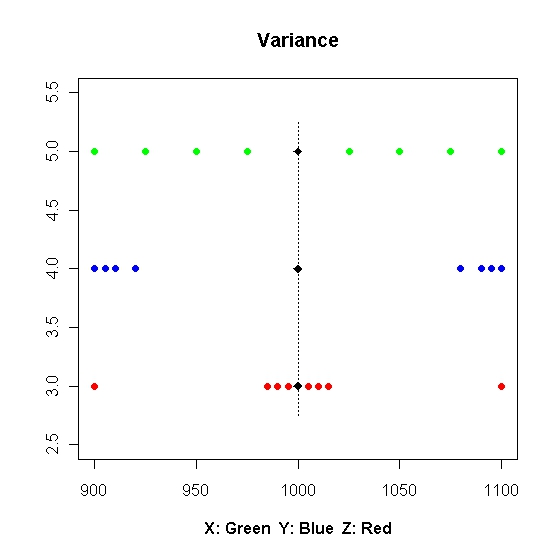
\includegraphics[scale=0.4]{2AVariance}
\end{center}

}

%--------------------------------------------------------%
\frame{
\frametitle{Variance}


\begin{itemize}

\item The (population) variance of a random variable is a non-negative number which gives an idea of how widely spread the values are likely to be; the larger the variance, the more scattered the observations on average.

\item Stating the variance gives an impression of how closely concentrated round the expected value the distribution is; it is a measure of the 'spread' of a distribution about its average value.

\item We distinguish between population variance (denoted $\sigma^2$) and sample variance (denoted $s^2$). For now, we will look only at sample variance.

\end{itemize}

}


%-------------------------------------------------------------------------%
\frame{

\frametitle{Sample Variance}

\begin{itemize}

\item Sample variance is a measure of the spread of or dispersion within a set of sample data.

\item The sample variance is the sum of the squared deviations from their mean divided by one less than the number of observations in the data set.

\item For example, for $n$ observations $x_1, x_2, x_3, \ldots , x_n$  with sample mean $\bar{x}$, the sample variance is given by


 \[ s^2 = { \sum (x-\bar{x})^2  \over n-1}\]




\end{itemize}
}
%--------------------------------------------------%
\frame{
\frametitle{Sample Standard Deviation}
\begin{itemize}
\item Standard deviation is the square root of variance
\item Standard deviation is commonly used in preference to variance because it is denominated in the same units as the mean.
\item For example, if dealing with time units, we could have a variance of something like $25$ \emph{ square minutes }, whereas the equivalent standard deviation is 5 minutes.
\item Population standard deviation is denoted  $\sigma$.
\item Sample standard deviation is denoted $s$.
\end{itemize}
}

%--------------------------------------------------------%
\begin{frame}[fragile]
\frametitle{Using \texttt{R}}Using \texttt{R} to compute standard deviation and variance for these data sets.

\begin{verbatim}
> X=c(900,925,950,975,1025,1050,1075,1100)
> Y=c(900,905,910,920,1080,1090,1095,1100)
> Z=c(900,985,990,995,1005,1010,1015,1100)
>
> sd(X);sd(Y);sd(Z)
[1] 73.19251
[1] 97.87018
[1] 54.37962
> 
>var(X);var(Y);var(Z)
[1] 5357.143
[1] 9578.571
[1] 2957.143
\end{verbatim}
\end{frame}

\end{document}

